%%
%% CORRECTNESS NOTIONS
%%
\section{Notions of Correctness for Consistency Specifications}
\label{chap:correctness:notions_correctness}

%\todo{Define correctness based on a networks adhering to the behavior of a multidirectional transformation}

%\todo{Korrektheit bx Netzwerk: es gib mx, deren Verhalten die bx emulieren müssen. Ist sehr stark, daher abschwächen. Ds muss nur kons. Zustand erreicht werden, egal wie? Einschränkung das original delta nicht geändert wird ist auch für mx künstlich.}

%\todo{Modular implies monolithic -> implicit correctness definition by implied relations}

\mnote{Different notions of correctness}
Before we formally define the above introduced artifacts, such as consistency relations, consistency preservation rules, an orchestration function and an application function, we first discuss different notions of \emph{correctness} for them.
Since there are different dimensions of correctness, we need to clarify which of them is relevant in the context of our research questions and will be defined in the formalization.

% \begin{definition}[Monolithic \ModelLevelConsistencyPreservationRule]
%     Given two metamodels $\metamodeltuple{M} = \tupled{\metamodelsequence{M}{n}}$ and a \modellevelconsistencyrelation between them $\consistencyrelation{CR}{} \subseteq \metamodelinstanceset{M}{1} \times \dots \times \metamodelinstanceset{M}{n}$.
%     A \emph{monolithic \modellevelconsistencypreservationrule} is a function:
%     \begin{align*}
%         \consistencypreservationrule{\consistencyrelation{CR}{}} : (\metamodeltupleinstanceset{M}, \metamodelinstanceset{M}{2}, \change{\metamodel{M}{1}}) \rightarrow \change{\metamodel{M}{2}}
%     \end{align*}
%     It that takes two consistent models and a change in the first one and returns a change in the second one.
%     We call a \modellevelconsistencypreservationrule \emph{correct} w.r.t. $\consistencyrelation{CR}{}$ if the resulting models when applying the input and output change are consistent to $\consistencyrelation{CR}{}$ again:
%     \begin{align*}
%         &
%         \forall \model{m}{1} \in \metamodelinstanceset{M}{1}, \model{m}{2} \in \metamodelinstanceset{M}{2} :
%         \tupled{\model{m}{1}, \model{m}{2}} \in \consistencyrelation{CR}{} \Rightarrow\\
%         & \formulaskip
%         \forall \change{\metamodel{M}{1}} \in \changeuniverse{\metamodel{M}{1}} :
%         \exists \change{\metamodel{M}{2}} \in \changeuniverse{\metamodel{M}{2}} :\\
%         & \formulaskip
%         \consistencypreservationrule{\consistencyrelation{CR}{}}(\model{m}{1}, \model{m}{2}, \change{\metamodel{M}{1}}) = \change{\metamodel{M}{2}} 
%         \land \tupled{\change{\metamodel{M}{1}}(\model{m}{1}), \change{\metamodel{M}{2}}(\model{m}{2})} \in \consistencyrelation{CR}{}
%     \end{align*}
% \end{definition}


\subsection{Relative Correctness Notions}

\mnote{Intuitive notion of correctness}
The overall objective regarding correctness of consistency preservation is to find models that are actually consistent.
Intuitively speaking, artifacts are correct if they fulfill their intended purpose. 
In our case, this means that consistency relations should consider models consistent whenever they are actually supposed to be considered consistent. 
Consistency preservation rules should return models that are actually consistent according to a consistency relation to be considered correct.
This also conforms to the notion of correctness for transformations, which realize consistency preservation rules, defined by \textcite{stevens2010sosym}.
And finally, the orchestration and application functions should execute the consistency preservation rules such that all models are consistent according to all relations afterwards.

\mnote{Correctness is relative}
Correctness of an artifact is usually considered with respect to some other specification, be it formally defined or only an informal notion.
For example, consistency relations may be supposed to be correct with respect to some informal notion of correctness that is collected by domain experts and requirements engineers.
A consistency preservation rule should always be consistent with respect to a consistency relation. As discussed before, this relation may either be defined explicitly and the preservation rule has to be correct with respect to it, or it may be induced by the fixed points of the preservation rule.
In the latter case, the consistency preservation rule will always be correct by construction.


\subsection{Correctness regarding Global Knowledge}

\mnote{Correctness of modular w.r.t. monolithic specification}
We previously distinguished between monolithic and modular notions of consistency.
In the above considerations, we relate the artifacts of a modular %(or in the special case also a monolithic) 
specification to each other.
Another notion of correctness can be defined by relating a modular artifact to a corresponding monolithic artifact.
For example, a set of modular consistency relations may be considered correct with respect to a monolithic relation when it considers the same tuples of models consistent.
For three metamodels $\metamodel{M}{1}, \metamodel{M}{2}, \metamodel{M}{3}$ with three modular consistency relations $\consistencyrelation{CR}{1,2}, \consistencyrelation{CR}{1,3}, \consistencyrelation{CR}{2,3}$ between them, as well as a ternary consistency relation $\consistencyrelation{CR}{1,2,3}$, we could say that $\consistencyrelation{CR}{1,2}, \consistencyrelation{CR}{1,3}, \consistencyrelation{CR}{2,3}$ are correct (with respect to $\consistencyrelation{CR}{1,2,3}$) if, and only if,
\begin{align*}
    & \forall \model{m}{1} \in \metamodel{M}{1}, \model{m}{2} \in \metamodel{M}{2}, \model{m}{3} \in \metamodel{M}{3}: \tupled{\model{m}{1}, \model{m}{2}, \model{m}{3}} \in \consistencyrelation{CR}{1,2,3} \\
    & \formulaskip
    \equivalent \tupled{\model{m}{1}, \model{m}{2}} \in \consistencyrelation{CR}{1,2} \land \tupled{\model{m}{1}, \model{m}{3}} \in \consistencyrelation{CR}{1,3} \land \tupled{\model{m}{2}, \model{m}{3}} \in \consistencyrelation{CR}{2,3}
\end{align*}
%
We may, analogously, define correctness for consistency preservation rules, an orchestration function, and an application function with respect to a single monolithic consistency preservation rule by defining that both deliver the same results for the same inputs or at least return a consistent result in the same cases.

\begin{figure}
    \centering
    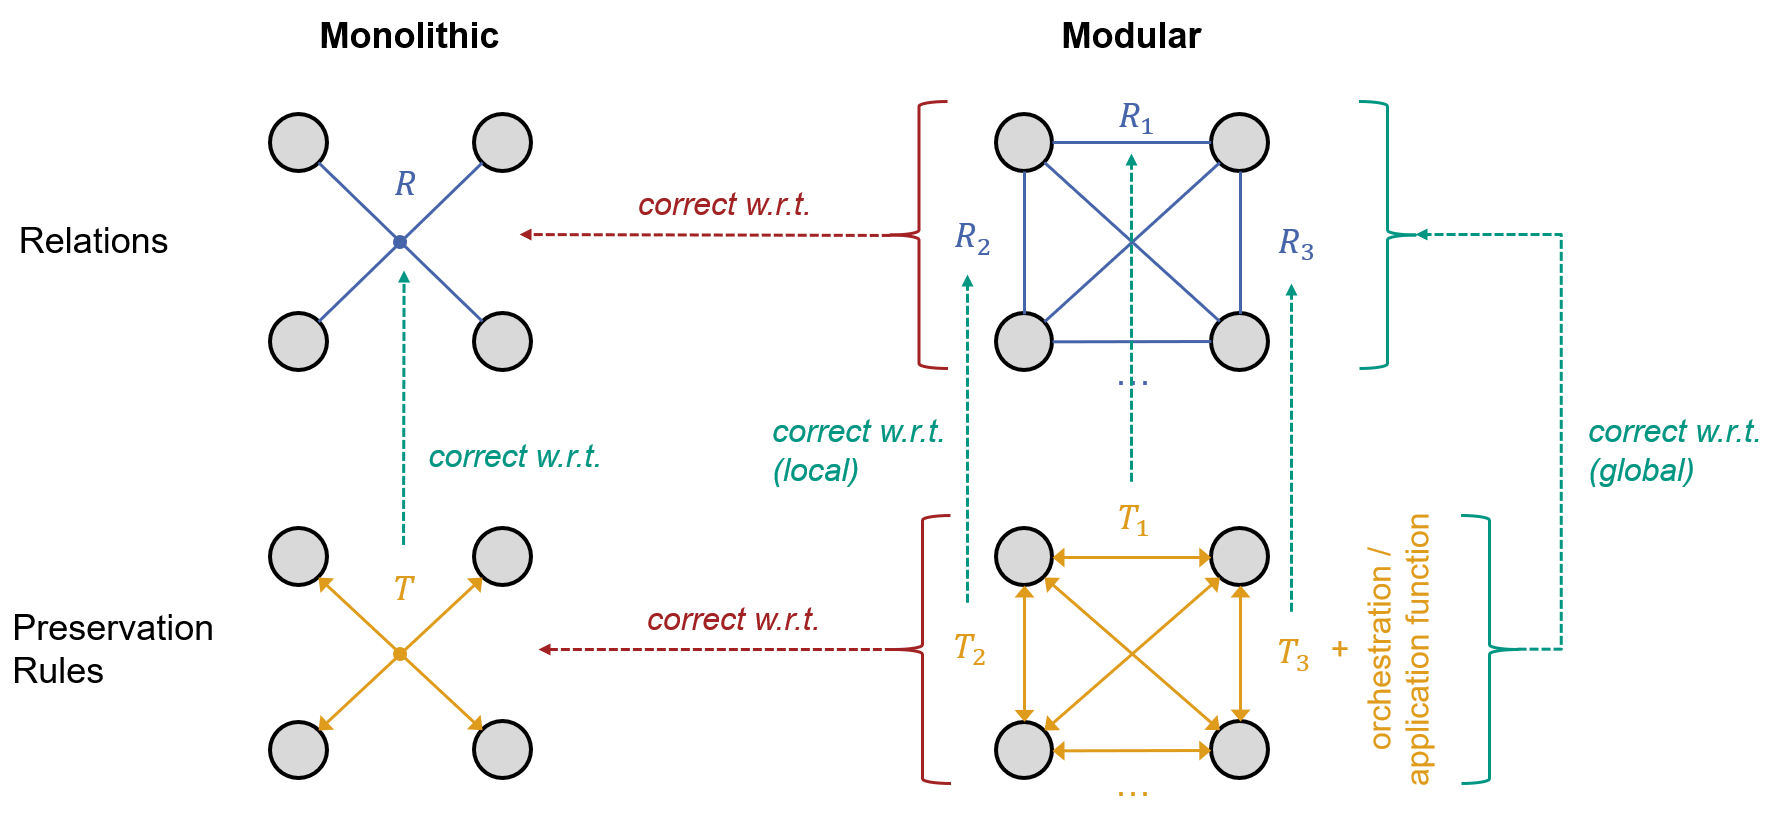
\includegraphics[width=\textwidth]{figures/correctness/notion/correctness_notions.png}
    \caption[Notions of correctness for consistency and its preservation]{Different notions of correctness for consistency and its preservation.}
    \label{fig:correctness:correctness_notions}
\end{figure}


\subsection{Dimensions of Correctness}
\label{chap:correctness:notions_correctness:dimensions}

\mnote{Two dimension of correctness notions}
The discussed correctness notions induce two dimensions: First, correctness can be considered between artifacts within a monolithic or modular specification. Second, correctness can be considered between artifacts of a modular specification and corresponding artifacts of a monolithic specification. These dimensions are depicted in \autoref{fig:correctness:correctness_notions}.
The former dimension is depicted vertically. Consistency preservation rules need to be correct with respect to their consistency relations.
In the modular case, in addition to each preservation rule being \emph{locally} correct with respect to its relation, the combination of preservation rules by means of an orchestration and application function must also be \emph{globally} correct with respect to the combination of all relations.
The latter dimension is depicted horizontally. Each modular artifact needs to be consistent with respect to a corresponding monolithic artifact.

\mnote{Drawbacks of global specification notions}
Although correctness of modular with respect to monolithic artifacts can be interesting from a theoretical perspective, its practical relevance is limited.
That notion of correctness assumes that there is some kind of global truth that has to be reflected by a modular specification.
This, however, has two essential drawbacks:
\begin{properdescription}
    \item[Validation Artifacts:] The artifacts to validate correctness against, i.e., the global, monolithic consistency relation as well as an appropriate monolithic consistency preservation rule, do usually not exist. If they existed, they could directly be used to preserve consistency. Thus, it is impossible to validate a set of consistency relations and consistency preservation rules against such a global specification.
    \item[Modular Knowledge:] This notion of correctness requires that the developers have some global knowledge that represents a monolithic consistency relation and its consistency preservation rule. As discussed before, we assume  the knowledge about relations between models to be usually distributed across several persons. Thus, there will not be such a global knowledge and not even an implicit notion of the necessary artifacts to validate the modular specifications against exists. % not to mention an explicit representation.
\end{properdescription}
%
Since this conflicts with our assumption of distributed knowledge about relations and independently developed, modular specifications, we do not further consider this notion of consistency.
In this thesis, we focus on correctness between the artifacts of a modular consistency specification.
We have discussed this correctness notion in more detail as correctness between a \emph{modularization level} and a \emph{global level} of consistency specification in previous work~\owncite{klare2019icmt}.


\subsection{Correctness of Consistency Relations}
\label{chap:correctness:notions_correctness:relations}

\mnote{Correctness of relations}
The consistency notion that we consider in the following especially requires that consistency preservation rules and the functions to orchestrate and apply them must be correct with respect to consistency relations.
This notion does, however, not define when consistency relations are considered \emph{correct}.
One option is to only consider correctness with respect to monolithic artifacts for the case of consistency relations, as we proposed in previous work~\cite{klare2019icmt}.
This, however, suffers from the discussed drawback of requiring a global notion of consistency.
Another notion of correctness would be conformance of the specified relations with what developers expect to be consistent, i.e., a validation of requirements.
For example, a consistency relation between UML and Java may only be considered correct if it fulfills some \enquote{natural} notion of consistency, as people know how elements are related because they represent similar things, such as classes, or because a standard like the \gls{UML}~\cite{uml} prescribes it.
In this work we do not consider such a correctness notion with respect to external, maybe not formally specified artifacts, as it is part of separate research on requirements engineering and validation.

\mnote{No correctness by construction}
In consequence, we might say that consistency relations are simply \emph{correct by construction}.
Thus, relations would normatively define what is to be considered consistent.
However, a consequence of not assuming a global knowledge of consistency is that different domain experts may have different and even conflicting notions of when models are to be considered consistent.
Consider for three metamodel $\metamodel{M}{1}, \metamodel{M}{2}, \metamodel{M}{3}$ the three modular consistency relations $\consistencyrelation{CR}{1,2} = \setted{\tupled{\model{m}{1},\model{m}{2}}}, \consistencyrelation{CR}{1,3} = \setted{\tupled{\model{m}{1},\model{m}{3}}}, \consistencyrelation{CR}{2,3} = \setted{\tupled{\model{m}{2},\model{m}{3}'}}$. 
Then there is no triple of models that is considered consistent to all relations. 
Although we still do not want to assume a global knowledge about consistency to which the modular one must conform, we might say that these relations are \emph{incompatible}, as we do not want to combine relations that induce an empty set of consistent model tuples.
Identifying an appropriate notion of \emph{compatibility} and how to check it constitutes \autoref{rq:correctness:compatibility} and will be discussed as our contribution \autoref{contrib:correctness:compatibility} in \autoref{chap:compatibility}.

\mnote{Induction of monolithic relation}
In fact, every set of modular consistency relations induces a monolithic one.
This monolithic relation $\consistencyrelation{CR}{}$ for metamodels $\metamodelsequence{M}{n}$ and pairwise consistency relations $\consistencyrelation{CR}{i,j}$ is defined by:
\begin{align*}
    \consistencyrelation{CR}{} = \setted{\tupled{\model{m}{1}, \dots, \model{m}{n}} \mid \bigwedge\limits_{1 \le i < j \le n} \tupled{\model{m}{i}, \model{m}{j}} \in \consistencyrelation{CR}{i,j}}
\end{align*}
At least if this induced relation is empty, we probably want to consider the modular relations incompatible, because if no models are considered consistent, we cannot describe any system consistently.


% Keeping multiple models consistent by means of transformations imposes either a single multidirectional transformation or a combination of several bi- or multidirectional transformations.
% Each of these transformations is able to take a consistent tuple of models and a change to them and to return a new consistent tuple of models.

% \mnote{Correctness implicitly covered by definitions}
% \textcite{stevens2010sosym} proposes an explicit notion of \emph{correctness} for transformations. This is based on the fact that her definition of a transformation does only specify that for two given model, which may be inconsistent because one was modified, an update of the other model is returned.
% The requirement that the originally modified model and the one returned by the transformation have to conform to some consistency relations is specified externally as a notion of \emph{correctness}.
% We directly relate a consistency preservation rule that restores consistency to an according consistency relation, thus a consistency preservation rule that follows our definition is correct by construction in terms of the correctness definition by \citeauthor{stevens2010sosym}.
% The same applies to the consistency preservation application function, which we consider \emph{correct} if it fulfills its definition, as that definition already covers all requirements to that function.

% \mnote{Different notions of correctness}
% In general, correctness can be considered in two ways: First, an artifact may be correct if it simply follows its definition.
% While for consistency relations, changes and the generic \modellevelconsistencypreservationrule generalization function correctness can be canonically achieved, this is not that simple for a consistency preservation rule and the consistency preservation application function, as they have to fulfill some constraints with respect to consistency relations they rely on.
% Second, an artifact may be correct if it fulfills some, maybe only implicitly known specification. For example, a consistency relation between UML and Java may only be considered correct if it fulfills some \enquote{natural} notion of consistency, as people know how elements have to be related because they represent similar things, such as classes, or because a standard like the UML~\cite{uml} prescribes that.

% \mnote{Correctness regarding global specifications}
% In this work we do not consider the latter correctness notion with respect to external, maybe not formally specified artifacts, which is part of separate research on validation.
% However, when considering consistency of multiple models it may be standing to reason that a modular specification of consistency and its preservation has to be correct with regards to some global, monolithic specification. More precisely, there may be a multiary relation putting several metamodels into relation, which the developers at least implicitly know, and a set of binary relations somehow has to respect that multiary relation, i.e., be \emph{correct} with respect to that relation.
% The same can be imagines for consistency preservation. One may define a multidirectional transformation for a multiary relation, taking a tuple of changes to consistent models and retuning a new tuple of changes, which applied to the models delivers a consistent set of models again. In fact, this would be a realization of the behavior of the consistency preservation application function without relying on modular \modellevelconsistencypreservationrules.

% \begin{description}
%     \item[Validation Artifacts:] The artifacts to check correctness against, i.e., the global, multiary consistency relation as well as an appropriate multidirectional transformation, do usually not exist. If they existed, they could directly be used to preserve consistency. Thus is impossible to validate a set of consistency relations and preservation rules against such a global specification.
%     \item[Modular Knowledge:] This notion of correctness requires that the developers have some global knowledge that represents a monolithic, multiary consistency relation and their preservation rules. Usually, this will not be the case, so there is even no implicit notion of the necessary artifacts to validate the modular specifications against, not to be mention an explicit representation.
% \end{description}

%\todo{Add an image for that relation}

% Overall Goals:
% \begin{itemize}
%     \item Define correctness of a transformation network: termination in consistent state
% \end{itemize}

